\documentclass[a4paper,12pt]{article}
\title{MATH1106 DIS207/208 Quiz 2}
\author{Benjamin Thompson}
\date{February 28, 2020}

\usepackage[margin=1in]{geometry}

\usepackage{amsmath}
\usepackage[usenames,dvipsnames]{xcolor}
\usepackage{tikz}
\usetikzlibrary{arrows.meta,decorations.markings}


\usepackage{pgfplots}

\pgfplotsset{every axis/.append style={
axis x line=middle,    % put the x axis in the middle
axis y line=middle,    % put the y axis in the middle
axis line style={-{Stealth[length=3mm]},color=black}, % arrows on the axis
minor tick num=1
            }}


\usepackage{fancyhdr}
\pagestyle{fancy}

\fancyhf{}
\lhead{MATH1106 DIS207/208 Quiz 2}
\rhead{February 28, 2020}
\cfoot{\thepage}

\usepackage{enumitem}

\newcommand{\bfa}{\mathbf{a}}
\newcommand{\bfb}{\mathbf{b}}
\newcommand{\bfc}{\mathbf{c}}
\newcommand{\bfd}{\mathbf{d}}


\begin{document}
\subsubsection*{Name:}
Each of the multiple choice questions below has one correct choice. Circle the correct choice.
\subsubsection*{Q1}
An SIR model for a system is created and described by the following equations.
\begin{align*}
S' &= \alpha S - \beta S - \gamma SI \\
I' &= \gamma SI - \beta I - \delta I \\
R' &= \delta I - \beta R - \rho R
\end{align*}
A mask program is introduced which significantly reduces the probablity of infection per encounter. Which of the coefficients above is likely to decrease?

\begin{enumerate}[label=(\alph*)]
\item $\beta$
\item $\gamma$
\item $\delta$
\item $\rho$
\end{enumerate}

\subsubsection*{Q2}
A $3$-dimensional vector field is described by the following equations.
\begin{align*}
	X' &= X - Y \\
	Y' &= Y - Z \\
	Z' &= Z - X
\end{align*}
(For example, the change vector at the point $(10,1,0)$ is $(9,1,-10)$). Which of the following statements regarding the vector field above is false?
\begin{enumerate}[label=(\alph*)]
\item The change vector at the point $(0,1,0)$ has the same length as the change vector at the point $(2,1,1)$.
\item The change vector at the point $(1,0,0)$ and the change vector at the point $(-1,0,0)$ have opposite directions.
\item The change vector at the point $(1,1,1)$ is a zero vector.
\item The change vector at the point $(0,1,0)$ is a unit vector.
\end{enumerate}

\subsubsection*{Q3}
The population of a feral buffalo herd in Australia\footnote{Yes, they were a serious problem in Australia in the 20th century.} is found to be described by
\[
	P' = P^2 - 4P.
\]
At time $t=4$ the population is $5$. Euler's method is used to estimate the population at time $t=6$ using the interval $\Delta t = 1$. This estimate is:

\begin{enumerate}[label=(\alph*)]
\item $60$
\item $70$
\item $80$
\item $90$
\end{enumerate}

\subsubsection*{Q4}
A line in the $xy$-plane with slope $5$ passes through the points $(3,2)$ and $(1,m)$. The value of $m$ is:
\begin{enumerate}[label=(\alph*)]
\item $-8$
\item $-4$
\item $4$
\item $8$
\end{enumerate}

\newpage

\subsubsection*{Q5}
The state space trajectory of a system with variables $M$, $N$ is shown below. Assuming that as time increases \emph{the trajectory goes in a counterclockwise direction}, which of the following graphs is a possible time-series of the trajectory? (Note: in the time-series graphs, the horizontal axis represents time.)
\[
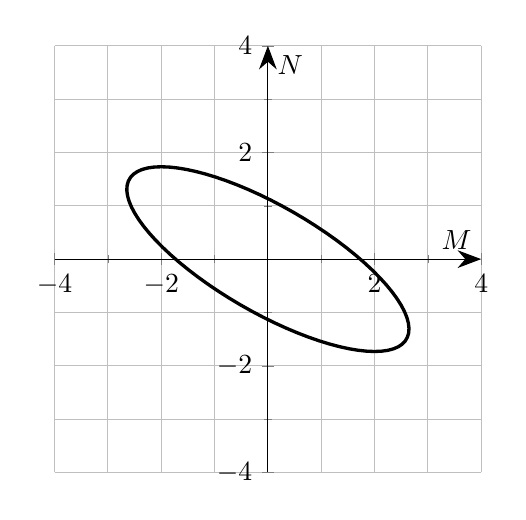
\begin{tikzpicture}
\begin{axis}[xlabel={$M$},ylabel={$N$},width=7cm, height=7cm, xmin=-4,xmax=4, ymin=-4,ymax=4, grid=both]
\addplot [very thick, domain=-4:4,samples=100]({3*cos(deg(x))*cos(-30) - 1*sin(deg(x))*sin(-30)},{3*cos(deg(x))*sin(-30) + 1*sin(deg(x))*cos(-30)}); 
\end{axis}
\end{tikzpicture}
\]
\[
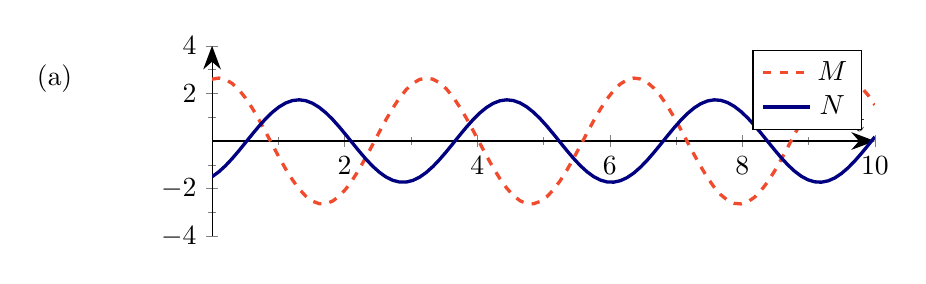
\begin{tikzpicture}

\begin{axis}[xlabel={$t$},width=10cm, height=4cm, xmin=0,xmax=10, ymin=-4,ymax=4, grid=none]
\addplot [dashed,RedOrange,very thick,domain=0:10,samples=100]{3*cos(2*deg(x))*cos(-30) - 1*sin(2*deg(x))*sin(-30)};
\addlegendentry{$M$}
\addplot [NavyBlue,very thick, domain=0:10,samples=100]{3*cos(2*deg(x))*sin(-30) + 1*sin(2*deg(x))*cos(-30)}; 
\addlegendentry{$N$}
\end{axis}

\node (a) at (-2,2) {(a)};
\end{tikzpicture}
\]
\[
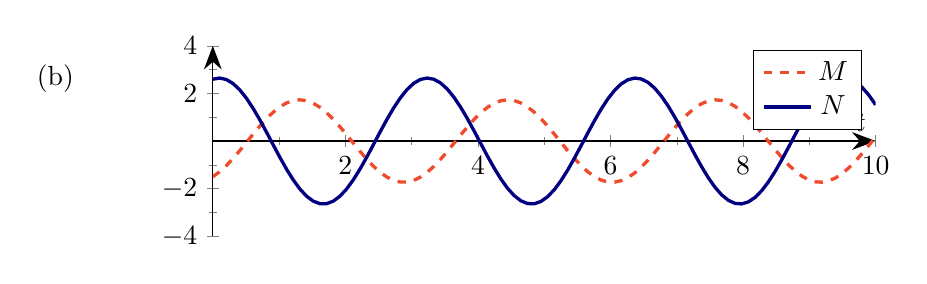
\begin{tikzpicture}

\begin{axis}[xlabel={$t$},width=10cm, height=4cm, xmin=0,xmax=10, ymin=-4,ymax=4, grid=none]
\addplot [dashed,RedOrange,very thick,domain=0:10,samples=100]{3*cos(2*deg(x))*sin(-30) + 1*sin(2*deg(x))*cos(-30)};
\addlegendentry{$M$}
\addplot [NavyBlue,very thick, domain=0:10,samples=100]{3*cos(2*deg(x))*cos(-30) - 1*sin(2*deg(x))*sin(-30)}; 
\addlegendentry{$N$}
\end{axis}

\node (b) at (-2,2) {(b)};
\end{tikzpicture}
\]
\[
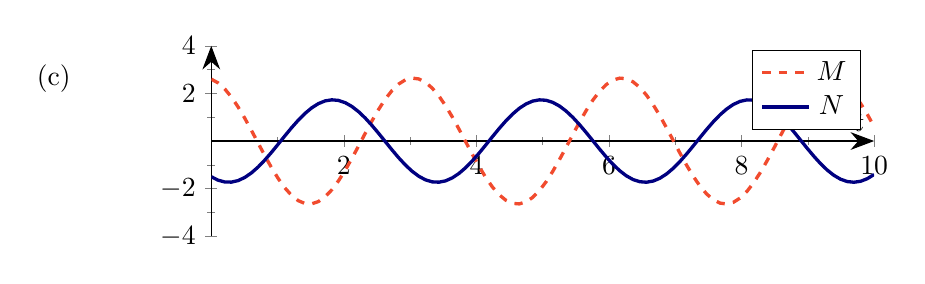
\begin{tikzpicture}

\begin{axis}[xlabel={$t$},width=10cm, height=4cm, xmin=0,xmax=10, ymin=-4,ymax=4, grid=none]
\addplot [dashed,RedOrange,very thick,domain=0:10,samples=100]{3*cos(2*deg(-x))*cos(-30) - 1*sin(2*deg(-x))*sin(-30)};
\addlegendentry{$M$}
\addplot [NavyBlue,very thick, domain=0:10,samples=100]{3*cos(2*deg(-x))*sin(-30) + 1*sin(2*deg(-x))*cos(-30)}; 
\addlegendentry{$N$}
\end{axis}

\node (c) at (-2,2) {(c)};
\end{tikzpicture}
\]
\[
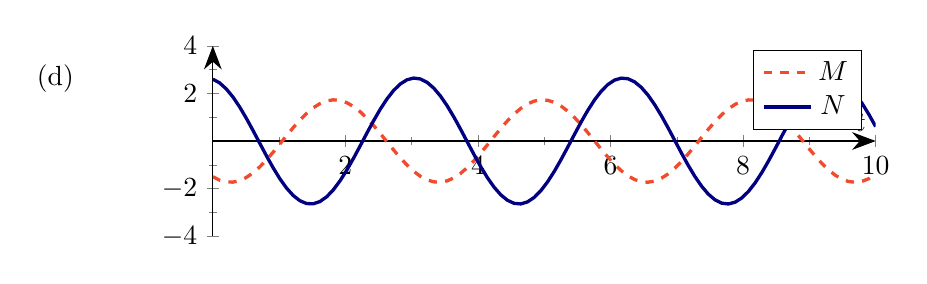
\begin{tikzpicture}

\begin{axis}[xlabel={$t$},width=10cm, height=4cm, xmin=0,xmax=10, ymin=-4,ymax=4, grid=none]
\addplot [dashed,RedOrange,very thick,domain=0:10,samples=100]{3*cos(2*deg(-x))*sin(-30) + 1*sin(2*deg(-x))*cos(-30)};
\addlegendentry{$M$}
\addplot [NavyBlue,very thick, domain=0:10,samples=100]{3*cos(2*deg(-x))*cos(-30) - 1*sin(2*deg(-x))*sin(-30)}; 
\addlegendentry{$N$}
\end{axis}

\node (d) at (-2,2) {(d)};
\end{tikzpicture}
\]

\end{document}
